\chapter{Statistical Analysis}
	To estimate the sensitivity of the $tH$ signal, we define an Asimov dataset, made by replacing the ensemble of simulated backgrounds and signal by a single one. The statistical uncertainty of the Asimov data is calculated as $\sqrt{n}$, with $n$ the number of events\cite{asimov}. The uncertainty of the signal strength is estimated by applying a fit to the Asimov dataset, where the model is constructed from the sum of the individual backgrounds and signal. The fit is implemented using a Poisson likelihood and Gaussian constraints for the systematical uncertainties in the model.
	
	\section{Likelihood and fit procedure}
	The likelihood function is the product of Poisson probabilities for all bins of the BDT distribution. The likelihood function has the form
	\begin{align}
		L(\mu,\alpha)=\prod_{j=1}^{N}\frac{(\mu s_j +b_j)^{n_j}}{n_j !}e^{-(\mu s_j+b_j)} \prod_{k=1}^M e^{\frac{-\alpha^2_k}{2}}
	\end{align}
	where $N$ is the total number of bins, $n_j$ is the number of events in a bin $j$, $s_j$ is the number of signal events, $\mu$ is a parameter that modifies the signal strength and $b_j$ is the number of background events.
	$b_j$ is the sum of different background processes $k$
	\begin{align}
		b_j=\sum_k^M b_j^k(1+ \alpha_k \sigma_k)
	\end{align}
	$\alpha_k$ is the parameter that modifies the expected background prediction and $\sigma_k$ is the systematic uncertainty of the associated background. $\sigma_k$ for the backgrounds are shown in the Table \ref{tth-table}.
	
	The fit is applied by minimizing the negative logarithm of the likelihood function (NLL) with respect to the parameter $\mu$ and $\alpha_k$. The minimization is performed by using programming language ROOT. ROOT is a scientific software toolkit, based on the C++ language, which main objective is the handling of data processing, statistical analysis, including visualization and storage. The package ROOFIT is used here, because of its implementations of modeling probability distributions and statistical tools\cite{roofit}. Figure \ref{simple} and Table \ref{table1}, shows the results of the fit to the Asimov data. 
	
	%log es usado para evitar valores extremadamente pequenos debido a los productos de los exponenciales
	%negativo es para hacer una minimizacion, positivo es maximizacion
	As mentioned before, for the $k_t$=-1 the number of events for signal is more than ten times compared to SM. This improves the sensitivity of the signal. Due to the small number of signal events the uncertainty for the SM is large compared to the $k_t$=-1 scenario, where the uncertainty is around 50$\%$. In this analysis only the signal is affected by the change $k_t$=1 (SM) $\rightarrow$ $k_t=-1$, therefore the backgrounds remain the same.
	
 Table \ref{parameters}, shows the $\mu$ and $\alpha$ parameters. For the pre-fit, values of $\alpha$ are set to zero and $\mu$ is set to 1. After the fit, $\alpha$ parameters set to zero indicates that in the fit, the values of the backgrounds did not change for the SM and the $\mu$ parameter set to 1 indicates that the signal strength also did not change.
	
	\pagebreak
	
		\begin{figure}[ht]
		\centering
		\begin{minipage}[b]{0.48\textwidth}
			\includegraphics[width=\textwidth]{Chapter4/simple.png}
		\end{minipage}
		\hfill
		\begin{minipage}[b]{0.48\textwidth}
			\includegraphics[width=\textwidth]{Chapter4/simple-kt-1.png}
		\end{minipage}
		\caption[Post-fit Signal and Backgrounds for $tH$ process]{Post-fit signal and background yields for $tH$ process for SM (Left) and $k_t=-1$ (Right).
			%In the box below each distribution, the ratio of the observed and predicted event yields is shown
		}
		\label{simple}
	\end{figure}
	\begin{table}[ht]
		\centering
		\caption[Post-fit yields for the fit to the Asimov data corresponding to 35.9 fb$^{-1}$]{Post-fit yields for the fit to the Asimov data corresponding to 35.9 fb$^{-1}$. The uncertainty given is the combined statistical plus systematic.}
		\begin{tabular}{ccc}
			\hline
			Process & SM & $k_{t}$=-1 \\
			\hline
			$t\bar{t}W$ & 68$\pm$8.9& 68 $\pm$8.9 \\
			$t\bar{t}Z$ & 25.9$\pm$3.8&25.9$\pm$3.8\\
			$WZ$ & 15.1$\pm$7.4& 15.1$\pm$7.4\\
			Rares & 20.8$\pm$4.8& 20.8$\pm$4.8 \\
			Fakes & 80.9$\pm$9.0& 80.9$\pm$8.9 \\
			$t\bar{t}H$ & 24.2$\pm$2.0 & 24.2$\pm$2.0 \\
			\hline
			$tH$& 2.1$\pm$16.5 &26.2$\pm$13.1 
		\end{tabular}
		\label{table1}
	\end{table}
	\begin{table}[ht!]
		\small
		\centering
		\caption{$\alpha$ and $\mu$ values for the fit to Asimov data corresponding to 35.9 fb $^{-1}$}
		\begin{tabular}{ccc}
			\hline
			Parameter & SM &$k_t$=-1\\
			\hline
			$\mu$ & 1.00 $\pm$ 7.74& 1.0 $\pm$ 0.5\\
			$\alpha_{t\bar{t}W}$& 0.00 $\pm$ 0.89& 0.00 $\pm$ 089\\
			$\alpha_{t\bar{t}Z}$ & 0.00 $\pm$ 0.98& 0.00 $\pm$ 0.98\\
			$\alpha_{WZ}$ & 0.00 $\pm$ 0.97& 0.00 $\pm$ 0.97\\
			$\alpha_{Rares}$ &0.00 $\pm$ 0.95&0.00 $\pm$ 0.98 \\
			$\alpha_{Fakes}$ & 0.00 $\pm$ 0.96& 0.00 $\pm$ 0.95\\
			$\alpha_{t\bar{t}H}$ &0.00 $\pm$ 0.98& 0.00 $\pm$ 0.98\\
		\end{tabular}
		\label{parameters}
	\end{table}
	
	\pagebreak

	\section{Limit calculation}
	Due to the large background, the signal strength for the Asimov data with 35.9 fb$^{-1}$ is consistent with zero.
	Therefore, we estimate an upper limit on the signal strength at 95$\%$ confidence level.
	
	We can define the likelihood ratio
	\begin{align}
		\lambda(\mu,\alpha)=\frac{L(\mu,\alpha)}{L(\hat{\mu},\hat{\alpha})}
	\end{align}
	Where $\hat{\alpha}$ and $\hat{\mu}$ are the parameters obtained in the previous section which correspond to the minimal of the NLL.
	To determine an upper limit on the strength parameter $\mu$, we use the following statistical test
	\begin{align}
		q(\mu,\alpha)= -2\ln{\lambda} 
	\end{align}
	High values of $q$ represent greater incompatibility between the data and the fit model.
	$q$ is a random variable with a $\chi^2$ distribution \cite{asimov}.

	\begin{figure}[ht]
		\centering
		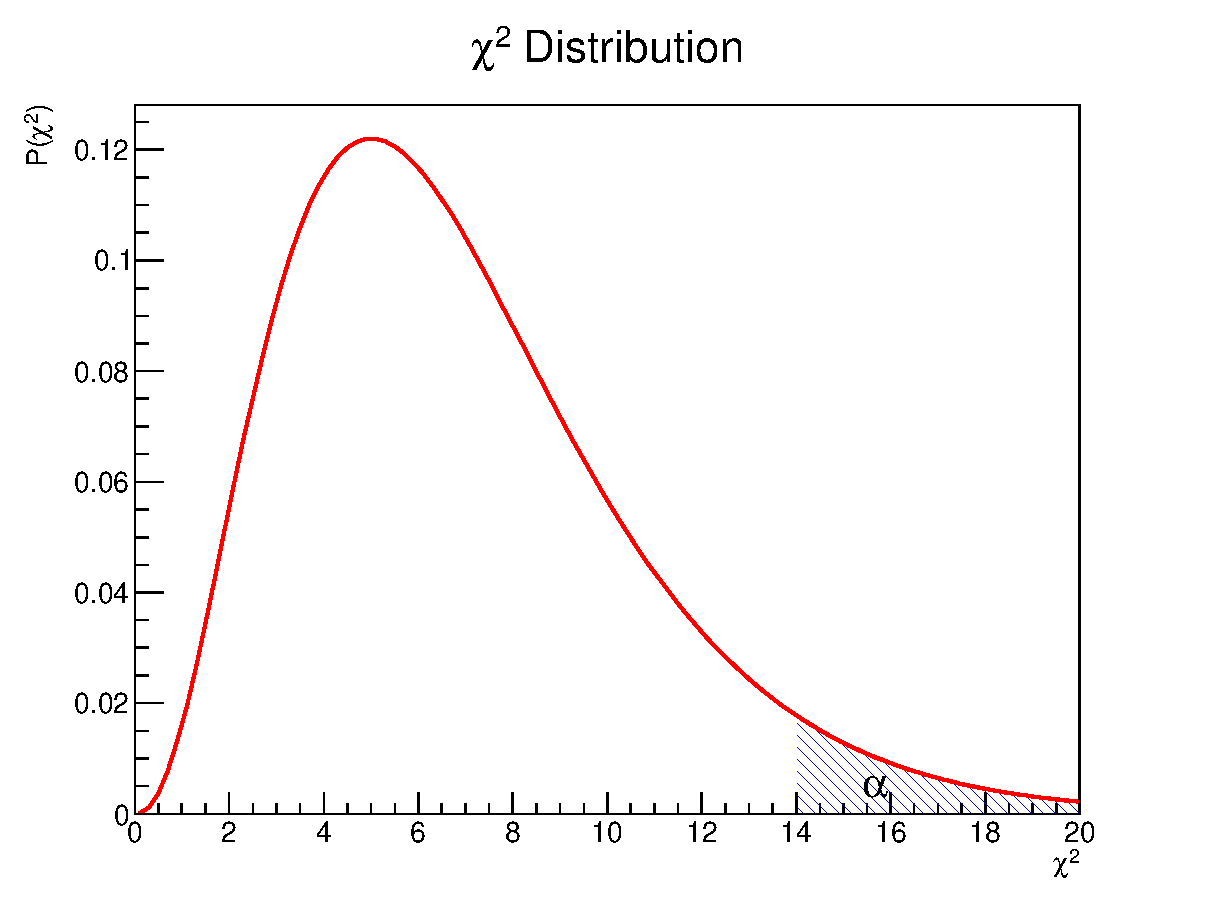
\includegraphics[scale=0.5]{Chapter4/chi}
		\caption[$\chi^2$ Distribution]{Illustration of the $\chi^2$ distribution with 7 degrees of freedom used for the limit estimation}
		\label{chi}
	\end{figure}
	
In order to find the upper limit value of $\mu$, we search for the largest value of $\mu$ such that $q$ remains below the shaded region shown in Figure \ref{chi}, where $\alpha$=0.05 in this case. It is useful to scan $q$ as function of $\mu$, which is normally a parabolic function as shown in Figure \ref{scanl}. In the SM case, the scan has a wider shape in comparison to the $k_t$=-1. This is due to larger statistical uncertainty on the $\mu$ parameter. 
	Using the above technique, we find an expected upper limit $\mu < $17.0 for SM model and $\mu < $ 2.3 for $k_t$=-1 model. 
		\begin{figure}[ht]
		\centering
		\begin{minipage}[b]{0.49\textwidth}
			\includegraphics[width=\textwidth,height=0.31\textheight]{Chapter4/Likelihood.png}
		\end{minipage}
		\hfill
		\begin{minipage}[b]{0.49\textwidth}
			\includegraphics[width=\textwidth,height=0.31\textheight]{Chapter4/Likelihood-kt-1.png}
		\end{minipage}
		\caption[Likelihood scan for SM and $k_t$=-1]{Likelihood scan for SM (Left) and $k_t$=-1 (Right).}
		\label{scanl}
	\end{figure}
	\pagebreak
	%%sigma son las probabilidades que corresponden a 1sigma=68, 2sigma=95, 3sigma=98 y sigma son los limites de la integral de una gaussiana
	\section{Extrapolation to higher luminosity}
	In the past section, it was shown that the signal strength with an integrated luminosity of 35.9 fb$^{-1}$ is not significant. The LHC has already collected data for integrated luminosity of 150 fb$^{-1}$ for run 2 which finished in 2018. Run 3 starts in 2021 and is expected an integrated luminosity of 300fb$^{-1}$ and for the high luminosity phase of LHC, expected to collect 3000 fb$^{-1}$. Therefore, it is interesting to study the sensitivity of the signal strength at higher luminosity. 
	An extrapolation (scale) is applied to the Asimov data and the statistical uncertainty is adjusted accordingly. For this analysis we assume the systematic uncertainties assigned to the background are the same.
	
	In Figure \ref{hm}, an estimated prediction of the signal and background events for higher luminosity is shown. As the luminosity increases, the number of events for both signal and backgrounds also increases, as previously explained in Chapter 1. But even with the increase of number of events, the statistical uncertainty of the data is too large with respect to the expected signal. In the likelihood scan for higher luminosity, as the luminosity increases, the relative uncertainty on the signal strength $\mu$ decreases. This is caused by the increased events available for the fit. 
	
	The same method is used for the model $k_t$=-1 in Figure \ref{hm1}. In this case, the number of events for the signal is more appreciable in comparison with the SM model. However, the likelihood scan parabolas are very closed and that indicates a decrease in the uncertainty of $\mu$ more notable than SM case. 
	Of course, as the previous section, we estimate the upper limit for these cases and they are shown in the Table \ref{upper}
	
		\begin{table}[ht]
		\caption[Results of $\mu$ and upper limits for SM and $k_t$=-1]{Results of $\mu$ and upper limits for Asimov extrapolations for SM  and $k_t$=-1 models at 95$\%$ confidence level.}
		\begin{tabular}{|c|c|c|c|c|}
			\hline
			\multirow{2}{*}{Luminosity (fb$^{-1}$)}  &\multicolumn{2}{c|}{SM ($k_t$=1)} &\multicolumn{2}{c|}{$k_t$=-1 scenario}\\
			\hhline{~----}	&$\mu$  &$\mu$ upper limit & $\mu$ &$\mu$ upper limit or interval\\
			\hline
			35.9 & 1.0 $\pm$ 7.7 & 17 & 1.0 $\pm$ 0.5 & 2.3 \\
			\hline
			150& 1.0 $\pm$ 6.7& 11 & 1.0 $\pm$ 0.4 &1.8\\
			\hline
			300&1.0 $\pm$ 4.3 &8.7 & 1.0 $\pm$ 0.3 &1.5 \\
			\hline
			3000&1.0 $\pm$ 1.7 & 4.3 &	 1.0 $\pm$ 0.1 & 0.9-1.1\\
			\hline
		\end{tabular}
		\label{upper}
	\end{table}
	
	
	However, the uncertainty of $\mu$ for the SM case is 170$\%$ for  in the 3000 fb$^{-1}$ case, making impossible to get an evidence of a Higgs boson in the $tH$ process for the same sign muon channel. Even at higher luminosity, the uncertainty of $\mu$ in SM case is still very big.
	In the $k_t$=-1 model the uncertainty of $\mu$ decreases with higher luminosity giving better results. This is caused by the fact that the number of events for the $tH$ signal is greater. For 3000 fb$^{-1}$ the uncertainty on $\mu$ is $~10\%$, and it has an upper limit that rounds between 0.9-1.1. In the likelihood scan, the statistical test $q$ gets very high values at $\mu$>1.1. This indicates that for large luminosity this model can be fully ruled out. This can be visualized in the likelihood scan of  3000 fb$^{-1}$, where the curve is very closed and values of $q$ are very high, giving incompatibility of the model with data.



	\pagebreak
	
	\begin{figure}[ht]
		\centering
		\begin{minipage}[b]{0.48\textwidth}
			\includegraphics[width=\textwidth]{Chapter4/150fb/simple-150.png}
		\end{minipage}
		\hfill
		\begin{minipage}[b]{0.5\textwidth}
			\includegraphics[width=\textwidth,height=0.31\textheight]{Chapter4/150fb/Likelihood.png}
		\end{minipage}
		\begin{minipage}[b]{0.48\textwidth}
			\includegraphics[width=\textwidth]{Chapter4/300fb/simple-300.png}
		\end{minipage}
		\hfill
		\begin{minipage}[b]{0.5\textwidth}
			\includegraphics[width=\textwidth,height=0.31\textheight]{Chapter4/300fb/Likelihood.png}
		\end{minipage}
		\begin{minipage}[b]{0.48\textwidth}
			\includegraphics[width=\textwidth]{Chapter4/3000fb/simple-3000.png}
		\end{minipage}
		\hfill
		\begin{minipage}[b]{0.5\textwidth}
			\includegraphics[width=\textwidth,height=0.31\textheight]{Chapter4/3000fb/Likelihood.png}
		\end{minipage}
		\caption{Fit and likelihood scan for 150 fb$^{-1}$, 300 fb$^{-1}$ and 3000 fb$^{-1}$ in SM}
		\label{hm}
	\end{figure}
	\pagebreak
	
	\begin{figure}[ht]
		\centering
		\begin{minipage}[b]{0.48\textwidth}
			\includegraphics[width=\textwidth]{Chapter4/kt-1/150fb/simple-150-kt-1.png}
		\end{minipage}
		\hfill
		\begin{minipage}[b]{0.48\textwidth}
			\includegraphics[width=\textwidth,,height=0.31\textheight]{Chapter4/kt-1/150fb/Likelihood.png}
		\end{minipage}
		\begin{minipage}[b]{0.48\textwidth}
			\includegraphics[width=\textwidth]{Chapter4/kt-1/300fb/simple-300-kt-1.png}
		\end{minipage}
		\hfill
		\begin{minipage}[b]{0.48\textwidth}
			\includegraphics[width=\textwidth,height=0.31\textheight]{Chapter4/kt-1/300fb/Likelihood.png}
		\end{minipage}
		\begin{minipage}[b]{0.48\textwidth}
			\includegraphics[width=\textwidth]{Chapter4/kt-1/3000fb/simple-3000-kt-1.png}
		\end{minipage}
		\hfill
		\begin{minipage}[b]{0.48\textwidth}
			\includegraphics[width=\textwidth,,height=0.31\textheight]{Chapter4/kt-1/3000fb/Likelihood.png}
		\end{minipage}
		\caption{Fit and likelihood scan for 150 fb$^{-1}$, 300 fb$^{-1}$ and 3000 fb$^{-1}$ in $k_t$=-1 model.}
		\label{hm1}
	\end{figure}
	
	
	%The Table shows the upper limits of $\mu$ for both models and different luminosities. For the SM case, the uncertainties in $\mu$ are greater than the $k_t$=-1 case. The increase of luminosity reduces the uncertainty of $\mu$ that is visualized in the likelihood graphs. 
	%The upper limits reduces as the luminosity increases; from 150 to 3000 fb $^{-1}$, the upper limit reduces in $\Delta\mu$=12.7 with $\Delta\mu$ the change of $\mu$.
	
	
	
	

